\article{Новости технологий}{Злобный янки в
3D-танке\\Полевые 3D-принтеры на службе американской армии}{

Пока специалисты в области 3D-печати рассуждают о перспективах приенения
технологии, а энтузиасты осторожно говорят о потенциальной возможности печати
необходимого скарба сразу на лунной базе (чтобы не тащить лишнее с Земли),
американская армия без всяких промедлений нашла применение 3D-печати уже сейчас.
Военные США стали использовать мобильные лаборатории Expeditionary Lab Mobile с
3D-принтерами в комплекте.

Основными задачами лабораторий Expeditionary Lab Mobile (сокращённо — ELM) будет
изготовление одноразовых инструментов для нужд армии, а также внесение
корректирующих дополнений в уже существующее оборудование — «полевое»
использование часто требует определённой доводки. В качестве примера приводится
случай, когда войска получают партию карманных фонарей с дефектом – быстро
выходящим из строя предохранителем выключателя. Находясь в кармане у военного,
такой фонарь может самопроизвольно включиться и либо выдать местонахождение
бойца, либо впустую разрядить батарейки. Однако, имея под рукой ELM, можно
быстро допечатать предохранители, без необходимости отсылки всей партии обратно
в США для замены.

\noindent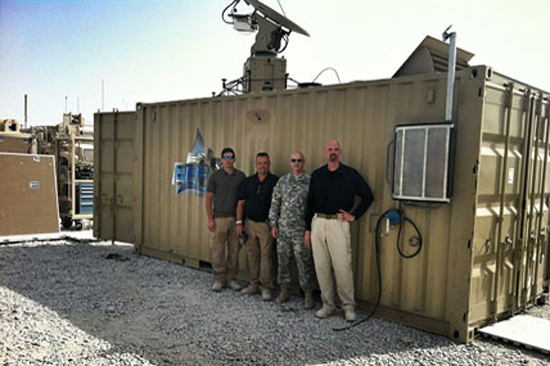
\includegraphics[width=\textwidth]{00/fig/yanky01.jpg}
\noindent\textbf{Чебураторы на тропе войны}

\begin{multicols}{2}
\noindent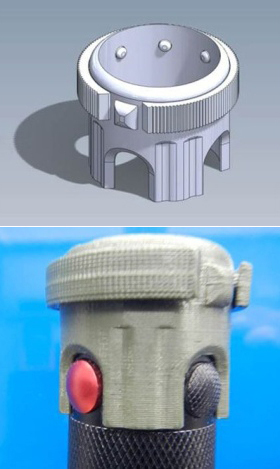
\includegraphics[width=0.8\columnwidth]{00/fig/yanky03.jpg}
\columnbreak
\noindent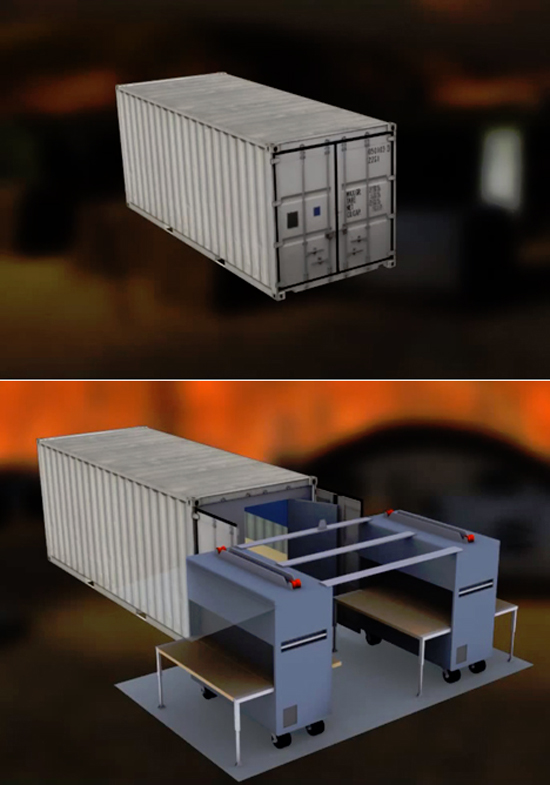
\includegraphics[width=0.8\columnwidth]{00/fig/yanky02.jpg}
\end{multicols}

Ещё одним примером можно назвать реальный случай недоработки в конструкции
миноискателя, приведший к тому, что время работы прибора из-за иракской жары
сократилось с восьми часов до 45 минут. В результате во время многодневных
миссий солдаты были вынуждены носить большое количество дополнительных батарей.
Использование ELM позволило сконструировать адаптер для использования батарей
другого типа и увеличить время работы миноискателя до девяти часов.

Expeditionary Lab Mobile представляет собой стандартный грузовой контейнер
(6,1$\times$2,4 м), внутри которого находятся 3D-принтер, специальные станки с
ЧПУ (для изготовления более сложных деталей из стали и алюминия) и набор
традиционных инструментов: резак, сварочный аппарат, циркулярная пила,
маршрутизатор, лобзик и сабельная пила. Кроме того, в комплекте ELM имеется
спутниковое оборудование связи для проведения телеконференций с чиновниками и
инженерами в США – для оперативных корректировок работы. При каждой лаборатории
будут находиться два инженера. Все лаборатории будут связаны между собой единой
компьютерной сетью.

Стоит отметить, что подобный способ изготовления износившихся или недостающих
деталей довольно дорог: стоимость каждой лаборатории составляет около 2,8
миллиона долларов. Планируется, что первые ELM будут испытаны в Афганистане.
Кроме того, можно надеяться, что успешное применение новых технологий на <<поле
боя>> будет способствовать их внедрению для мирных операций. Например, во время
стихийных бедствий.

}{\copyright\
\href{http://www.computerra.ru/50860/polevyie-3d-printeryi-na-sluzhbe-amerikans/}{Компьютерра, Николай Маслухин}
}

